\documentclass[11pt]{article}
\usepackage[margin=0.9in]{geometry}
\usepackage[T1]{fontenc}
\usepackage{lmodern}
\usepackage{amsmath,amssymb}
\usepackage{tikz}
\usepackage{listings}
\usepackage{enumitem}
\usepackage{xcolor}
\usepackage{needspace}

\definecolor{pastc}{HTML}{1F5FA8}
\definecolor{newc}{HTML}{B5521B}
\definecolor{codebg}{HTML}{F6F6F6}

\lstset{language=C++, basicstyle=\ttfamily\small, numbers=left, numberstyle=\tiny\color{gray},
  columns=fullflexible, keepspaces=true, backgroundcolor=\color{codebg}, frame=single,
  rulecolor=\color{gray!40}, xleftmargin=1.5em, framexleftmargin=1.5em}

\tikzset{bst/.style={level distance=1.1cm, every node/.style={circle,draw,minimum size=7mm,inner sep=0pt}}}

\newcounter{qnum}
\newcommand{\tagpast}[1]{\colorbox{pastc}{\textcolor{white}{\footnotesize\textbf{PAST EXAM}}}\ {\footnotesize\textcolor{pastc}{(#1)}}}
\newcommand{\tagnew}[1]{\colorbox{newc}{\textcolor{white}{\footnotesize\textbf{NEW -- SIMILAR PATTERN}}}\ {\footnotesize\textcolor{newc}{(modeled on #1)}}}
% \question{title}{tag}
\newcommand{\question}[2]{\par\needspace{8\baselineskip}\medskip\stepcounter{qnum}%
  \noindent\textbf{\theqnum.\ #1}\hfill #2\par\nobreak\smallskip}
\newcommand{\answer}[2]{\par\medskip\noindent\textbf{#1}\quad Answer: \textbf{#2}\par\nobreak\smallskip}
\newenvironment{choices}{\begin{enumerate}[label=\textbf{\Alph*)}, nosep, leftmargin=2.5em]}{\end{enumerate}}

\begin{document}

\begin{center}
{\Large\textbf{EECS 281 --- Exam 2 Practice Questions}}\\[3pt]
Sorting $\cdot$ Quicksort $\cdot$ Hash Tables $\cdot$ Trees $\cdot$ AVL
\end{center}

\noindent Questions tagged \tagpast{source} are copied word for word from the Fall 2026 Exam 2 practice exam.
Questions tagged \tagnew{source} are new, written to follow the same patterns with different numbers and twists.
Answers are on the last pages.

% =====================================================================
\section*{Part I --- Multiple Choice}

% ---------------- Q1 ----------------
\question{Quicksort}{\tagpast{Practice Exam 2, Q2}}
Suppose we run quicksort on the following list $[\,4, 12, 9, 1, 2, 5, 3, 8, 7\,]$. We choose the last element, 7,
as the pivot. After partitioning as described in lecture (but \textbf{before} we run the recursive function calls),
what is the resulting list?
\begin{choices}
  \item $[\,4, 3, 5, 1, 2, 7, 12, 9, 8\,]$
  \item $[\,4, 3, 5, 1, 2, 9, 12, 8, 7\,]$
  \item $[\,4, 3, 1, 5, 2, 7, 12, 8, 9\,]$
  \item $[\,4, 3, 5, 1, 2, 7, 12, 8, 9\,]$
\end{choices}

% ---------------- Q2 ----------------
\question{Quicksort Partition}{\tagnew{Practice Exam Q2}}
Suppose we run quicksort on the array $[\,8, 3, 14, 6, 11, 2, 9, 1, 13, 7\,]$, choosing the last element, $7$, as the pivot.
After one call to \texttt{partition()} as described in lecture (code below, called on the range \texttt{[0, 10)}),
but \textbf{before} the recursive calls, what is the resulting array?
\begin{lstlisting}
int32_t partition(std::vector<int32_t>& vec, int32_t left, int32_t right) {
  int32_t pivot = --right;
  while (true) {
    while (vec[left] < vec[pivot]) ++left;
    while (left < right && vec[right - 1] >= vec[pivot]) --right;
    if (left >= right) break;
    std::swap(vec[left], vec[right - 1]);
  } // while
  std::swap(vec[left], vec[pivot]);
  return left;
} // partition()
\end{lstlisting}
\begin{choices}
  \item $[\,3, 6, 2, 1, 7, 14, 9, 8, 13, 11\,]$
  \item $[\,1, 3, 2, 6, 7, 14, 9, 8, 13, 11\,]$
  \item $[\,1, 3, 2, 6, 7, 11, 14, 9, 8, 13\,]$
  \item $[\,3, 6, 2, 1, 7, 8, 14, 11, 9, 13\,]$
\end{choices}

% ---------------- Q3 ----------------
\question{Sorting}{\tagnew{Practice Exam Q1 \& Q11}}
Which of the following statements is \textbf{true}?
\begin{choices}
  \item Heapsort is stable, and its worst-case time complexity is $\Theta(n\log n)$.
  \item If every element of an array is at most $k$ positions away from its final sorted position,
        insertion sort runs in $O(nk)$ time on that array.
  \item Quicksort as described in lecture (last element as pivot) runs in $\Theta(n\log n)$ time on an
        array that is already sorted.
  \item Mergesort is adaptive: on an already-sorted array it runs in $\Theta(n)$ time.
  \item Because insertion sort runs in $\Theta(n)$ on sorted input, it is possible to design a comparison
        sort whose worst-case time on arbitrary input is $\Theta(n)$.
\end{choices}

% ---------------- Q4 ----------------
\question{Collision Resolution}{\tagpast{Practice Exam 2, Q4}}
You are given a hash table with size $M = 10$ and hash function $H(n) = (2n + 3) \bmod M$. Collisions
are resolved using quadratic probing. What would the table look like (with an X denoting an empty
location) after inserting the following elements in the order given? Use $c_1 = 0$ and $c_2 = 1$.
\[ 4,\ 10,\ 12,\ 7,\ 2 \]
\begin{choices}
  \item $[X, 4, X, 10, X, X, X, 12, 7, 2]$
  \item $[X, 4, 2, 10, X, X, X, 12, 7, X]$
  \item $[X, 4, X, 10, X, X, 2, 12, 7, X]$
  \item $[X, 4, X, 10, X, X, 2, 12, X, 7]$
\end{choices}

% ---------------- Q5 ----------------
\question{Collision Resolution}{\tagnew{Practice Exam Q4}}
A hash table has size $M = 11$ and primary hash function $t(k) = k \bmod 11$. Collisions are resolved with
double hashing: the $j$-th probe ($j = 0, 1, 2, \ldots$) examines index $\big(t(k) + j \cdot t'(k)\big) \bmod 11$,
where $t'(k) = 7 - (k \bmod 7)$. Erasing a key replaces it with a \emph{deleted} marker (tombstone).
Duplicates are not allowed. To insert, probe as in a search (continuing past deleted slots) until the key is found
(no insertion) or an empty slot is reached. Then place the key in the \emph{first} deleted or empty slot seen.
Perform these operations in order:
\[ \text{insert } 35,\ 40,\ 24,\ 72,\ 79;\quad \text{erase } 35;\quad \text{insert } 24;\quad \text{insert } 34 \]
What does the table look like afterward? (X = empty, DEL = deleted.)
\begin{choices}
  \item \texttt{[X, 34, DEL, 24, 79, X, 72, 40, X, X, X]}
  \item \texttt{[72, 79, DEL, 34, X, X, 24, 40, X, X, X]}
  \item \texttt{[72, 79, 34, X, X, X, 24, 40, X, X, X]}
  \item \texttt{[72, 79, 24, 34, X, X, 24, 40, X, X, X]}
\end{choices}

% ---------------- Q6 ----------------
\question{Tree ADT}{\tagpast{Practice Exam 2, Q7}}
What does the following function return?
\begin{lstlisting}
int count(Node* curNode) {
  if (curNode == nullptr)
    return 0;
  else if (curNode->parent == nullptr)
    return 1 + count(curNode->left) + count(curNode->right);
  else if (curNode->left == nullptr && curNode->right == nullptr)
    return 1;
  else
    return count(curNode->left) + count(curNode->right);
} // count()
\end{lstlisting}
\begin{choices}
  \item The number of nodes in the tree
  \item The number of internal nodes
  \item The number of external (leaf) nodes
  \item The number of external (leaf) nodes plus the root
  \item The depth of the tree
\end{choices}

% ---------------- Q7 ----------------
\question{Tree ADT}{\tagnew{Practice Exam Q7}}
Using \texttt{struct Node \{ int val; Node *left; Node *right; \};}, what does \texttt{mystery(root, k)} return
for $k \ge 0$? The root is at depth 0.
\begin{lstlisting}
int mystery(Node *node, int k) {
  if (node == nullptr)
    return 0;
  if (k == 0)
    return (node->left == nullptr && node->right == nullptr) ? 1 : 0;
  return mystery(node->left, k - 1) + mystery(node->right, k - 1);
} // mystery()
\end{lstlisting}
\begin{choices}
  \item The number of nodes at depth exactly $k$
  \item The number of leaf nodes at depth at most $k$
  \item The number of leaf nodes at depth exactly $k$
  \item The number of internal (non-leaf) nodes at depth exactly $k$
  \item The number of leaf nodes in the entire tree, regardless of $k$
\end{choices}

% ---------------- Q8 ----------------
\question{Tree Traversal}{\tagpast{Practice Exam 2, Q8}}
Given the following preorder and inorder traversals of a binary tree, what is the postorder traversal of this
same binary tree?
\begin{itemize}[nosep]
  \item Preorder: 11, 19, 31, 7, 10
  \item Inorder: 31, 19, 11, 10, 7
\end{itemize}
\begin{choices}
  \item 11, 19, 7, 31, 10
  \item 31, 19, 10, 7, 11
  \item 19, 31, 10, 7, 11
  \item 31, 10, 7, 19, 11
  \item 10, 7, 31, 19, 11
\end{choices}

% ---------------- Q9 ----------------
\question{Tree Traversal}{\tagnew{Practice Exam Q8}}
Given the following postorder and inorder traversals of a binary tree, what is the \emph{preorder} traversal of the same tree?
\begin{itemize}[nosep]
  \item Postorder: 27, 15, 9, 4, 21, 6, 30, 12
  \item Inorder: 27, 4, 15, 9, 12, 30, 21, 6
\end{itemize}
\begin{choices}
  \item 12, 4, 27, 9, 15, 30, 6, 21
  \item 12, 30, 6, 21, 4, 9, 15, 27
  \item 12, 4, 27, 9, 15, 30, 21, 6
  \item 12, 4, 30, 27, 9, 6, 15, 21
  \item 12, 4, 27, 15, 9, 30, 21, 6
\end{choices}

% ---------------- Q10 ----------------
\question{AVL Trees}{\tagpast{Practice Exam 2, Q10}}
Which of the following statements about AVL trees is \textbf{true}?
\begin{choices}
  \item Optimally re-balancing an AVL tree after a deletion can take more than $O(1)$ time.
  \item For an insert operation, up to three rotations are needed.
  \item Searching an AVL tree can take longer than $O(\log n)$.
  \item Given an $n$-node binary search tree that has never been balanced, the BST can be made into a
        balanced AVL tree using $O(\log n)$ rotations.
  \item A tree is AVL balanced if and only if the absolute difference in heights of the root's children is less than 2.
\end{choices}

% ---------------- Q11 ----------------
\question{Insertion/Deletion}{\tagpast{Practice Exam 2, Q12}}
Given the following AVL tree:
\begin{center}
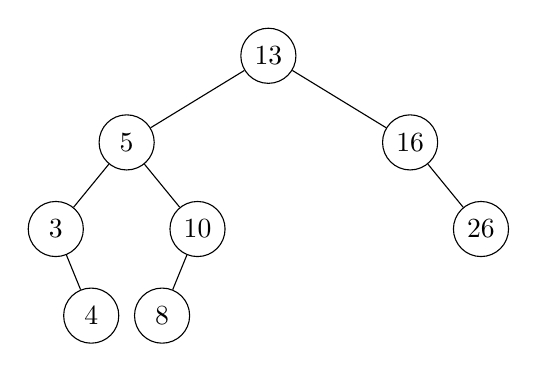
\begin{tikzpicture}[bst, level 1/.style={sibling distance=3.6cm}, level 2/.style={sibling distance=1.8cm},
  level 3/.style={sibling distance=0.9cm}]
\node {13}
  child {node {5}
    child {node {3} child[missing] child {node {4}}}
    child {node {10} child {node {8}} child[missing]}}
  child {node {16}
    child[missing]
    child {node {26}}};
\end{tikzpicture}
\end{center}
Perform the following operations:
\begin{enumerate}[nosep]
  \item Delete 13 (replace with its inorder successor)
  \item Insert 9
\end{enumerate}
What are the left and right children of ``16'' after performing the operations?
\begin{choices}
  \item 8, 26
  \item 9, 26
  \item 10, 26
  \item \texttt{nullptr}, 26
  \item \texttt{nullptr}, \texttt{nullptr}
\end{choices}

% ---------------- Q12 ----------------
\question{Insertion/Deletion}{\tagnew{Practice Exam Q12}}
Given the following AVL tree:
\begin{center}
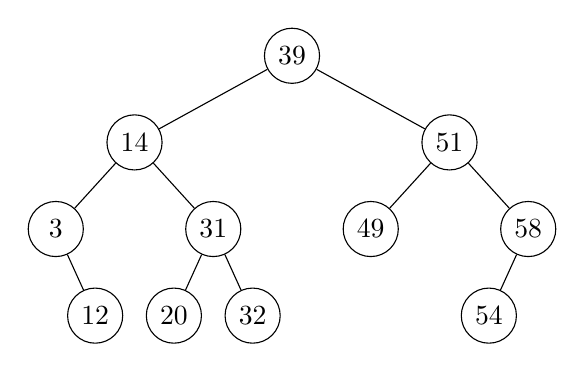
\begin{tikzpicture}[bst, level 1/.style={sibling distance=4cm}, level 2/.style={sibling distance=2cm},
  level 3/.style={sibling distance=1cm}]
\node {39}
  child {node {14}
    child {node {3} child[missing] child {node {12}}}
    child {node {31} child {node {20}} child {node {32}}}}
  child {node {51}
    child {node {49}}
    child {node {58} child {node {54}} child[missing]}};
\end{tikzpicture}
\end{center}
Perform the following operations, rebalancing with AVL rotations after each one:
\begin{enumerate}[nosep]
  \item Delete 39 (replace it with its inorder successor)
  \item Insert 33
\end{enumerate}
What are the left and right children of ``49'' after performing the operations?
\begin{choices}
  \item 14, 51
  \item 14, 54
  \item 33, \texttt{nullptr}
  \item 32, 54
  \item 14, 58
\end{choices}

% =====================================================================
\newpage
\section*{Part II --- Written}

% ---------------- Q13 ----------------
\question{Programming: Counting in a Range [8 Points]}{\tagnew{Practice Exam Q13}}
Using the following definition of a binary tree node:
\begin{lstlisting}
struct Node {
  int val;
  Node *left;
  Node *right;
};
\end{lstlisting}
\texttt{node} is the root of a binary search tree with distinct values. Implement \texttt{countInRange()}, which returns
the number of values $v$ in the tree with $\texttt{lo} \le v \le \texttt{hi}$. You may assume $\texttt{lo} \le \texttt{hi}$.

\smallskip\noindent\textbf{Requirements:} Your solution must run in $O(h + k)$ time, where $h$ is the height of the tree
and $k$ is the value returned. You may use up to $O(h)$ auxiliary space. (A solution that visits every node,
$\Theta(n)$, will not receive full credit.)

\smallskip\noindent\textbf{Implementation:} Limit: 10 lines of code. You may use any C, C++, or STL function/algorithm.
\begin{lstlisting}
int countInRange(Node *node, int lo, int hi) {
\end{lstlisting}

% ---------------- Q14 ----------------
\question{Programming: Inserting into a Hash Table [12 Points]}{\tagnew{Practice Exam Q14}}
Given the following definition of a hash table structure:
\begin{lstlisting}
enum class Status { Empty, Occupied, Deleted };
struct HashTable {
  std::vector<int> buckets;
  std::vector<Status> status;
};
\end{lstlisting}
The table resolves collisions with quadratic probing. Let $M$ be the table size (\texttt{buckets.size()}) and
$h(\texttt{val}) = \texttt{val} \bmod M$. You may assume $\texttt{val} \ge 0$. The $i$-th probe ($i = 0, 1, \ldots, M-1$)
examines index $\big(h(\texttt{val}) + c_1 i + c_2 i^2\big) \bmod M$. Use $c_1 = 2$ and $c_2 = 1$.
Erased values are marked \texttt{Deleted} (tombstones), and the set allows no duplicates.

Implement \texttt{insert()}. If \texttt{val} is already in the table, return \texttt{false} without changing the table.
Otherwise, store \texttt{val} in the \emph{first} \texttt{Deleted} or \texttt{Empty} slot encountered while probing,
mark it \texttt{Occupied}, and return \texttt{true}. As in lecture, a \texttt{Deleted} slot does \emph{not} end the
search, but an \texttt{Empty} slot does. If the $M$ probes reach no \texttt{Empty} slot, do not find \texttt{val}, and
pass no \texttt{Deleted} slot, return \texttt{false}.

\smallskip\noindent\textbf{Requirements:} Your solution must implement quadratic probing. It must run in $O(M)$ time
and use $O(1)$ auxiliary space.

\smallskip\noindent\textbf{Implementation:} Limit: 20 lines of code. You may use any C, C++, or STL function/algorithm.
\begin{lstlisting}
bool insert(HashTable &tbl, int val) {
\end{lstlisting}

% =====================================================================
\newpage
\section*{Answer Key}

\answer{1. Quicksort (past)}{D}
Pivot $=7$. \texttt{L} moves right while $v[L] < 7$; \texttt{R} moves left while $v[R-1] \ge 7$; swap; repeat.
\begin{itemize}[nosep]
  \item \texttt{L} stops at 12, \texttt{R} stops at 3 $\Rightarrow$ $[4,3,9,1,2,5,12,8,7]$
  \item \texttt{L} stops at 9, \texttt{R} stops at 5 $\Rightarrow$ $[4,3,5,1,2,9,12,8,7]$
  \item \texttt{L} stops at 9 (index 5), \texttt{R} meets \texttt{L} $\Rightarrow$ swap 9 with the pivot: $[4,3,5,1,2,7,12,8,9]$
\end{itemize}

\answer{2. Quicksort Partition (new)}{B}
\begin{itemize}[nosep]
  \item \texttt{L} stops at 8 (index 0); \texttt{R} skips 13 and stops at 1 $\Rightarrow$ $[1,3,14,6,11,2,9,8,13,7]$
  \item \texttt{L} stops at 14 (index 2); \texttt{R} skips 8, 9 and stops at 2 $\Rightarrow$ $[1,3,2,6,11,14,9,8,13,7]$
  \item \texttt{L} stops at 11 (index 4); \texttt{R} skips 14, 11 and meets \texttt{L} $\Rightarrow$ swap 11 with pivot:\\ \hspace*{1em}$[1,3,2,6,7,14,9,8,13,11]$
\end{itemize}
Distractors: A is Lomuto partitioning, C shifts the pivot into place instead of swapping, and D is a stable partition.

\answer{3. Sorting (new)}{B}
For insertion sort, each element only has to shift past larger elements that started before it. All of those lie within
$2k$ positions, so the work is $O(k)$ per element and $O(nk)$ total.
(A) Heapsort is \emph{not} stable.
(C) On sorted input the last element is always the max, so the splits are $n-1$ and $0$, giving $\Theta(n^2)$.
(D) Mergesort is $\Theta(n\log n)$ in every case.
(E) Comparison sorts need $\Omega(n\log n)$ comparisons in the worst case, since $\log_2(n!)$ comparisons are needed.

\answer{4. Collision Resolution (past)}{C}
Probe index $= (H(n) + i^2) \bmod 10$.
4 $\to 11 \bmod 10 = 1$.\ \
10 $\to 3$.\ \
12 $\to 7$.\ \
7 $\to 7$ (taken), $7+1=8$.\ \
2 $\to 7$ (taken), 8 (taken), $7+4=11\to1$ (taken), $7+9=16\to6$.
Result: $[X,4,X,10,X,X,2,12,7,X]$.

\answer{5. Collision Resolution (new)}{C}
$35\to2$. \ $40\to7$. \ $24\to2$ (taken), $t'=4$: slot 6. \ $72\to6$ (taken), $t'=5$: $11\bmod11=0$. \
$79\to2$ (taken), $t'=5$: 7 (taken), $12\bmod11=1$.
Erase 35: slot 2 becomes DEL.
Insert 24: slot 2 is DEL, so keep probing; 24 is found at slot 6, so nothing changes.
Insert 34: $34\bmod11=1$ (taken), $t'(34)=1$: slot 2 is DEL (remember it), slot 3 is empty, so 34 is absent. Place it in the
first DEL slot, slot 2.
Result: \texttt{[72, 79, 34, X, X, X, 24, 40, X, X, X]}.
Distractors: A uses linear probing, B does not reuse the tombstone, and D stops the search at DEL, which inserts a duplicate 24.

\answer{6. Tree ADT (past)}{D}
A leaf returns 1. A non-root internal node adds nothing of its own; it only sums its children. The root adds
$1$ on top of its subtrees. So the function counts the leaves, plus one for the root.

\answer{7. Tree ADT (new)}{C}
Each call moves one level down and decreases $k$, so $k$ reaches 0 exactly at depth $k$. Only those nodes can contribute,
and only if they are leaves. Shallower nodes add nothing (there is no ``$1+$''), and the recursion never goes deeper than $k$.

\answer{8. Tree Traversal (past)}{B}
The root is 11. Inorder splits into left $\{31,19\}$ and right $\{10,7\}$.
The left preorder is $19,31$, so 19 has left child 31. The right preorder is $7,10$, so 7 has left child 10.
Postorder: $31,19,10,7,11$.

\answer{9. Tree Traversal (new)}{A}
The last postorder entry, 12, is the root. Inorder gives left $\{27,4,15,9\}$ and right $\{30,21,6\}$.
Left: its postorder is $27,15,9,4$, so 4 is the root, with left child 27 and right child 9, and 9 has left child 15.
Right: its postorder is $21,6,30$, so 30 is the root, with right child 6, and 6 has left child 21.
Preorder: $12,4,27,9,15,30,6,21$.
Distractors: B is the reversed postorder, D is the level order, and C and E use the \emph{first} postorder element as the root.

\answer{10. AVL Trees (past)}{A}
A deletion can trigger a rotation at every level on the way up, i.e.\ $O(\log n)$ rotations.
(B) An insert needs at most one single or one double rotation.
(C) AVL height is $\Theta(\log n)$, so search is $O(\log n)$.
(D) A degenerate chain needs $\Omega(n)$ rotations.
(E) \emph{Every} node must be balanced, not just the root.

\answer{11. Insertion/Deletion (past)}{B}
\textbf{Delete 13:} the successor 16 moves to the root and 26 takes 16's old spot. The root is now $+2$ and its left child 5 has
balance $0$, so do a \emph{single} right rotation. Result: $5\big(3(\varnothing,4),\ 16(10(8,\varnothing),\,26)\big)$.\\
\textbf{Insert 9:} 9 becomes 8's right child. Node 10 is $+2$ with child 8 at $-1$ (the LR case), so do a double rotation: 9 replaces 10,
with children 8 and 10. 16's children are now \textbf{9 and 26}.
(A double rotation on the delete step, which is wrong when the child's balance is 0, leads to D.)

\answer{12. Insertion/Deletion (new)}{D}
\textbf{Delete 39:} the successor 49 (a leaf) moves to the root. Now 51 has balance $-2$, and its right child 58 is $+1$ (the RL case):
rotate right at 58, then left at 51, giving $54(51,58)$.
The tree is $49\big(14(3(\varnothing,12),\,31(20,32)),\ 54(51,58)\big)$.\\
\textbf{Insert 33:} 33 becomes 32's right child. The root 49 is now $+2$ (left height 3 vs.\ right height 1), and its left child 14 is
$-1$ (the LR case). Rotate left at 14, then right at 49.
The final tree is $31\big(14(3(\varnothing,12),20),\ 49(32(\varnothing,33),\,54(51,58))\big)$, so 49's children are \textbf{32 and 54}.
Distractors: A skips rebalancing entirely, B skips rebalancing after the insert, C uses the predecessor, and E uses a single rotation on the delete.

\answer{13. Counting in a Range (new)}{reference solution}
\begin{lstlisting}
int countInRange(Node *node, int lo, int hi) {
  if (node == nullptr) return 0;
  if (node->val < lo) return countInRange(node->right, lo, hi); // prune left
  if (node->val > hi) return countInRange(node->left, lo, hi);  // prune right
  return 1 + countInRange(node->left, lo, hi) + countInRange(node->right, lo, hi);
} // countInRange()
\end{lstlisting}
Every visited node is either in range (at most $k$ of them) or on the search path for \texttt{lo} or for \texttt{hi} (at most $2(h+1)$ of them).
That gives $O(h+k)$ time, plus $O(h)$ recursion stack. Common deductions: a full traversal; recursing into both children when
the node is out of range; off-by-one errors with \texttt{<} vs.\ \texttt{<=}.

\needspace{25\baselineskip}
\answer{14. Inserting into a Hash Table (new)}{reference solution}
\begin{lstlisting}
bool insert(HashTable &tbl, int val) {
  size_t M = tbl.buckets.size(), home = static_cast<size_t>(val) % M;
  size_t target = M;  // first Deleted/Empty slot seen (M = none yet)
  for (size_t i = 0; i < M; ++i) {
    size_t idx = (home + 2 * i + i * i) % M;  // c1 = 2, c2 = 1
    if (tbl.status[idx] == Status::Empty) {
      if (target == M) target = idx;
      break;  // Empty ends the search: val is not in the table
    }
    if (tbl.status[idx] == Status::Deleted) {
      if (target == M) target = idx;  // remember it, but keep probing
    } else if (tbl.buckets[idx] == val) {
      return false;  // already present
    }
  }
  if (target == M) return false;  // no usable slot on the probe sequence
  tbl.buckets[target] = val;
  tbl.status[target] = Status::Occupied;
  return true;
} // insert()
\end{lstlisting}
Two traps. (1) Stopping at the first \texttt{Deleted} slot: \texttt{val} may be further along the probe sequence, so this
creates duplicates. (2) Not reusing tombstones: the key must go in the \emph{first} \texttt{Deleted} or \texttt{Empty} slot.
Also, never compare \texttt{buckets[idx]} on a \texttt{Deleted} slot, because the stale value is still stored there.
There are at most $M$ probes with $O(1)$ work each, so time is $O(M)$ and extra space is $O(1)$.

\end{document}
